%
%===============>>  ГРУППА 7-1 МОДУЛЬ 4  <<=============
%
\setmodule{4}
%
%===============>>  Занятие 1  <<===============
%
\begin{class}[number=1]
	\begin{listofex}
		\item Разделить число:
		\begin{enumcols}[itemcolumns=3]
			\item \( 15 \) в отношении \( 2:3 \)
			\item \( 120 \) в отношении \( 5:7 \)
			\item \( 54 \) в отношении \( 3:2:4 \)
		\end{enumcols}
		\item Точка \( K \) лежит на отрезке \( AB \) , \( AB=6 \) см, причём \( AK \) больше
		\( BK \) на \( 4,6 \) см. Найдите длины отрезков \( AK \) и \( BK \).
		\item Отрезок \( AB=14 \) см. Точка \( M \) делит этот отрезок в отношении \( AM:MB=3:4 \). Чему равны длины отрезков \( AM \) и \( MB \)?
		\item Точка \( C \) делит отрезок \( AB \) в отношении \( 4:5 \). Найдите длину \( AB \), если \( BC=10 \).
		\item Отрезок \( AB=14 \), а \( BC \) в \( \mfrac{1}{2}{7} \) раза больше отрезка \( AB \). Найдите \( AB+BC \).
		\item На прямой отложили отрезок \( AB=6 \) см. За точку \( B \) на прямой отметили точку \( C \) так, что \( AC \) в \( 4 \) раза больше, чем \( AB \). Найдите длину \( BC \).
		\item Точка \( B \) делит отрезок \( AC \) в отношении \( AB:BC=2:1 \). Точка \( D \) делит отрезок \( AB \) в отношении \( AD:DB=3:2 \). В каком отношении точка \( D \) делит отрезок \( AC \)?
		\item Решить уравнение:
		\begin{enumcols}[itemcolumns=3]
			\item \( 3x-12=4(x-1) \)
			\item \( 0,25(x-2)=15-0,75x \)
			\item \( 2x(x-15)+24=2x^2-6x \)
		\end{enumcols}
	\end{listofex}
\end{class}
%
%===============>>  Занятие 2  <<===============
%
\begin{class}[number=2]
	\begin{listofex}
		\item Разделить число:
		\begin{enumcols}[itemcolumns=3]
			\item \( 22 \) в отношении \( 5:6 \)
			\item \( 200 \) в отношении \( 13:7 \)
			\item \( 36 \) в отношении \( 7:3:2 \)
		\end{enumcols}
		\item Точки \( O \),\( K \),\( M \) лежат на одной прямой. Найти расстояние между
		точками \( O \) и \( M \) , если \( OK = 8,2 \) см, \( KM = 7,3 \) см. Указать все
		возможные решения.
		\item Боковая сторона равнобедренного треугольника равна \( 12 \), а периметр треугольника равен \( 44 \). Найдите длину основания.
		\item Точка \( K \) делит отрезок \( AB \) в отношении \( AK:BK=3:7 \). Найдите длину \( AB \), если \( BK=21 \).
		\item Отрезок \( AB=11 \), а \( BC \) в \( 1,7 \) раза больше отрезка \( AB \). Найдите \( BC-AB \).
		\item Сумма двух сторон равнобедренного треугольника равна \( 26 \) см, а
		периметр равен \( 36 \) см, какими могут быть стороны этого
		треугольника?
		\item Решить пропорцию:
		\begin{enumcols}[itemcolumns=2]
			\item \( 3:7,5=x:\mfrac{6}{1}{4}\)
			\item \( \dfrac{x}{1,8}=\dfrac{2,7}{0,09} \)
		\end{enumcols}
	\end{listofex}
\end{class}
%
%===============>>  Домашняя работа 1  <<===============
%
\begin{homework}[number=1]
	\begin{listofex}
		\item Разделить число:
		\begin{enumcols}[itemcolumns=3]
			\item \( 30 \) в отношении \( 4:2 \)
			\item \( 70 \) в отношении \( 3:4 \)
			\item \( 150 \) в отношении \( 9:4:2 \)
		\end{enumcols}
		\item Вычислить:
		\begin{enumcols}[itemcolumns=3]
			\item \( \dfrac{15^5}{3^4\cdot5^6} \)
			\item \( 3,5\cdot(8,68+1,136)-135,531:33,3 \)
		\end{enumcols}
		\item Решить пропорцию:
		\begin{enumcols}[itemcolumns=2]
			\item \( x:51,6=11,2:34,4 \)
			\item \( \dfrac{12,3}{6}=\dfrac{x}{4,2} \)
		\end{enumcols}
		\item Боковая сторона равнобедренного треугольника равна \( 13 \), а периметр треугольника равен \( 50 \). Найдите длину основания.
		\item Решить уравнение:
		\begin{enumcols}[itemcolumns=2]
			\item \( 17x+2=4(4x-23) \)
			\item \( 0,2(x-2,5)=7,5-1,8x \)
		\end{enumcols}
	\end{listofex}
\end{homework}
%
%===============>>  Занятие 3  <<===============
%
\begin{class}[number=3]
	\begin{listofex}
		\item Прямой угол поделили в отношении \( 7:3 \). Найдите величины получившихся частей.
		\item Развернутый угол поделили в отношении \( 1:2 \) и в каждой части провели биссектрису. Найдите угол между биссектрисами. Изменится ли результат, если отношение \( 1:2 \) заменить на \( 2:3 \)? Проверить и пояснить результат.
	\end{listofex}
	\begin{definit}
		Сумма углов в треугольнике равна \( 180\degree \).
	\end{definit}
	\begin{listofex}
		\item В треугольнике \( ABC \) угол \( \angle A = 80\degree \) и \( \angle B = 30\degree \). Найдите величину угла \( \angle C \).
		\item В треугольнике \( ABC \) угол \( \angle A \) в две раза меньше угла \( \angle B \) и в три раза меньше угла \( \angle C \). Найдите все углы треугольника \( ABC \).
		\item Два угла в треугольнике \( ABC \) в сумме составляют \( 150\degree \) и относятся друг к другу как \( 7:8 \). Найдите эти углы, а также третий угол треугольника \( ABC \).
		\item Все три угла в треугольнике \( ABC \) относятся друг к другу как \( 1:2:15 \). Найдите углы треугольника \( ABC \).
	\end{listofex}
	\begin{definit}
		В равнобедренном треугольнике прилегающие к основанию углы равны.
	\end{definit}
	\begin{listofex}[resume]
		\item Угол \( B \) при основании \( AB \) равнобедренного треугольника \( ABC \) равен \( 34\degree \). Найдите, чему равен угол при вершине треугольника \( ABC \).
		\item Угол при вершине равнобедренного треугольника в два раза меньше, чем угол при основании. Найдите углы треугольника.
		\item Решить уравнение:
		\begin{enumcols}[itemcolumns=2]
			\item \( 26x+2(x-1)=3(7x-10) \)
			\item \( 0,01(x-3,2)=1,034-0,12x \)
		\end{enumcols}
	\end{listofex}
\end{class}
%
%===============>>  Занятие 4  <<===============
%\begin{class}[number=4]
%	\begin{listofex}
%		\begin{enumcols}
%			\item Пусто
%		\end{enumcols}
%	\end{listofex}
%\end{class}
%
%===============>>  Домашняя работа 2  <<===============
%
\begin{homework}[number=2]
		\begin{listofex}
			\item В равнобедренном треугольнике \(ABC\) с основанием \(AC\) внешний угол при вершине \(C\) равен \(123 \degree \). Найдите величину угла \(ABC\). Ответ дайте в градусах.
			\item В треугольнике \( ABC \) угол \( \angle A \) в два раза больше угла \( \angle B \) и в три раза меньше угла \( \angle C \). Найдите все углы треугольника \( ABC \).
			\item Все три угла в треугольнике \( ABC \) относятся друг к другу как \( 2:7:11 \). Найдите углы треугольника \( ABC \).
			\item Два угла в треугольнике \( ABC \) в сумме составляют \( 135\degree \) и относятся друг к другу как \( 7:8 \). Найдите эти углы, а также третий угол треугольника \( ABC \).
			\item Развернутый угол поделили в отношении \( 6:4 \) и в каждой части провели биссектрису. Найдите угол между биссектрисами.
			\item Угол при вершине равнобедренного треугольника больше на \(20 \degree\), чем угол при основании. Найдите все углы треугольника.
			\item Решить уравнения:
			\begin{enumcols}[itemcolumns=2]
				\item \( x-2(2x-7)=2x \)
				\item \( 4x-2(3x+5)=0,5(4x-3) \)
				\item \( 0,6x=5 \cdot (0,1x-6) \)
				\item \( 0,01(8-2x)=1,5-0,7x \)
		\end{enumcols}
	\end{listofex}
\end{homework}
%
%===============>>  Занятие 5  <<===============
%
\begin{class}[number=5]
	\begin{definit}
		Периметр --- это сумма длин всех сторон фигуры.
	\end{definit}
	\begin{listofex}
		\item В треугольнике \(ABC\) \(AB = 5\), \(AC\) в два раза больше чем \( AB \), \(BC = 9\). Найдите периметр треугольника \( ABC \).
		\item Сумма двух сторон равнобедренного треугольника равна \( 20 \) см, а периметр равен \( 28 \) см, какими могут быть стороны этого треугольника.
		\item Найди длину прямоугольника, если его ширина \(7\) см, а периметр равен \(40\) см.
		\item Сторона квадрата \(18\) см. Найди длину прямоугольника с таким же периметром и шириной \(14\) см.
	\end{listofex}
	\begin{definit}
		Равными называются фигуры, которые при наложении совпадают.
	\end{definit}
	\begin{definit}
		Если две стороны и угол между ними одного треугольника соответственно равны двум сторонам и углу между ними другого треугольника, то такие треугольники равны.
	\end{definit}
	\begin{listofex}[resume]
		\item
		\begin{minipage}[t]{0.63\linewidth}
			Дан четырехугольник \( ARTV \). Известно, что \( RT=AV \) и \( \angle RTA = \angle TAV \). Докажите что треугольники \( ART \) и \( AVT \) равны.
		\end{minipage}
		\hspace{0.03\linewidth}
		\begin{minipage}[c]{0.34\linewidth}
			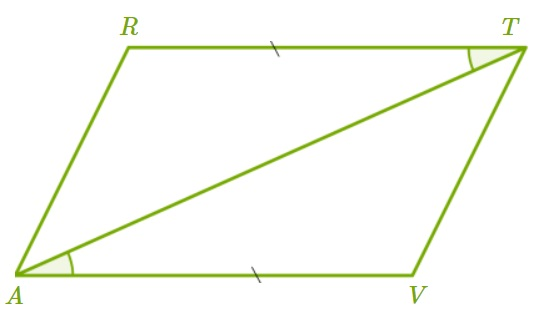
\includegraphics[width=\linewidth]{pics/G71M4C5-3.jpg}
		\end{minipage}
		\item Докажите, что серединный перпендикуляр, проведенный к основанию равнобедренного треугольника, делит этот треугольник на два равных.
		\item
		\begin{minipage}[t]{0.73\linewidth}
			Дан прямоугольник \(GHEF\), докажите что треугольники \(HEO\) и \(GOF\) равны, и \(GOH\) с \(EOF\).
		\end{minipage}
		\hspace{0.03\linewidth}
		\begin{minipage}[c]{0.24\linewidth}
			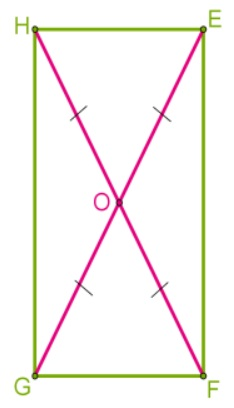
\includegraphics[width=0.7\linewidth]{pics/G71M4C5-1.jpg}
		\end{minipage}
		\item
		\begin{minipage}[t]{0.45\linewidth}
			Точка пересечения \( O \) делит каждый из отрезков \( AD \) и \( TM \) пополам. Найдите углы \(A\) и \(T\), если угол \(M = 22 \degree\), а угол \(D = 57 \degree\).
		\end{minipage}
		\hspace{0.05\linewidth}
		\begin{minipage}[t]{0.5\linewidth}
			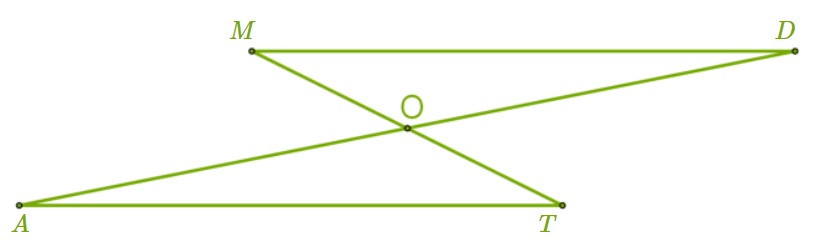
\includegraphics[align=t, width=\textwidth]{pics/G71M4C5-2.jpg}
		\end{minipage}
		\item Вычислить: \( \left( \mfrac{5}{7}{12}-\mfrac{3}{17}{36} \right)\cdot\mfrac{2}{1}{2}+\mfrac{4}{1}{3}\cdot\dfrac{3}{26}+\dfrac{1}{2} \)
		\item Сумма двух чисел равна \(2,4\), а их разность равна \(1,63\). Найдите эти числа.
	\end{listofex}
\end{class}
%
%===============>>  Домашняя работа 3  <<===============
%
%\begin{homework}[number=2]
%	\begin{listofex}
%
%	\end{listofex}
%\end{homework}
%\newpage
%\title{Подготовка к проверочной работе}
%\begin{listofex}
%	
%\end{listofex}
%
%===============>>  Занятие 6  <<===============
%
\begin{class}[number=6]
	\begin{listofex}
		\item Вычислите периметр равнобедренного треугольника \(АВС\), если \(D\) - точка пересечения медианы угла \(А\) и основания треугольника, а периметр треугольника \(ADC\) равен \(18\) cм, и \(CD = 6\) cм и \(AD = BD\).
		\item Сторона \(CD\) треугольника \(CDE = 24\) см, сторона \(CE\) в \(3\) раза меньше стороны  \(CD\), а сторона \(DE\) на \(7\) см больше стороны \(CD\). Найти периметр треугольника  \(CDЕ\).
		\item Периметр треугольника равен \(62\) см, а одна из сторон равна \(21\) см. Найти две другие стороны, если одна из них на \(5\) см больше другой.
		\item Может ли периметр треугольника быть равным \(19\), если одна из его сторон на \(1\) короче другой и на \(3\) длиннее третьей?
		\item Диагонали \(AC\) и \(BD\) четырехугольника \(ABCD\) пересекаются в точке \(O\). Периметр треугольника \(ABC\) равен периметру треугольника \(ABD\), а периметр треугольника \(ACD\) --- периметру треугольника \(BCD\). Докажите, что \(AO = BO\).
		\item Докажите, что если диагонали четырёхугольника делят друг друга пополам, то противоположные стороны четырёхугольника - равны.
		\item Докажите, что в равных треугольниках соответствующие высоты равны между собой.
		\item На сторонах \(BC\) и \(B_1C_1\) равных треугольников \(ABC\) и \(A_1B_1C_1\) взяты соответственно точки \(M\) и \(M_1\), причем \(BM : MC = B_1M_1 : M_1C_1\). Докажите, что \(AM = A_1M_1\).
		\item Медиана треугольника делит его на два треугольника, периметры которых равны. Докажите, что треугольник равнобедренный.
	\end{listofex}
\end{class}
%
%
%===============>>  Занятие 7  <<===============
%
%\begin{class}[number=7]
%	\begin{listofex}
%		
%	\end{listofex}
%\end{class}
%
%===============>>  Провечная работа  <<===============
%
%\begin{exam}
%	\begin{listofex}
%	
%	\end{listofex}
%\end{exam}